\documentclass[a4paper]{scrreprt}

\usepackage[ngerman]{babel}
\usepackage[utf8]{inputenc}
\usepackage[T1]{fontenc}
\usepackage{lmodern}

\usepackage[german,linesnumbered,algoruled,longend,vlined]{algorithm2e}
\DontPrintSemicolon
\SetArgSty{}
\SetKw{KwOr}{or}
\SetKw{KwAnd}{and}
\SetKw{KwNot}{not}
\setlength{\algomargin}{3ex}

\usepackage[fixlanguage]{mybabelbib}
% \selectlanguage{ngerman}
\setbibliographyfont{title}{}
\setbibliographyfont{jtitle}{}
\setbibliographyfont{btitle}{\emph}
\setbibliographyfont{stitle}{\emph}
\setbibliographyfont{journal}{\emph}

\usepackage{amsmath}
\usepackage{amsfonts}
\usepackage{amssymb}
\usepackage{amsthm}

\usepackage{graphicx}
\usepackage[a4paper,bookmarks,bookmarksnumbered]{hyperref}
\usepackage[font=small,format=hang,labelfont=bf,figurename=Abb.,tablename=Tab.]{caption}
\usepackage{enumerate}

\newtheorem{satz}{Satz}[chapter]
\newtheorem{lemma}[satz]{Lemma}
\newtheorem{beobachtung}[satz]{Beobachtung}
\newtheorem{folgerung}[satz]{Folgerung}
\newtheorem{korollar}[satz]{Korollar}
\theoremstyle{definition}
\newtheorem{definition}[satz]{Definition}
\newenvironment{beweis}{\begin{proof}}{\end{proof}}

\graphicspath{{abbildungen/}}

\begin{document}
%%%%%%%%%%%%%%%%%%%%%%%%%%%%%%%%%%%%%%%%%%%%%%%%%%%%%%%%%%%%%%%%%%%%%%%%%%
%%%%%%%%%%%%% Bitte nur ab hier Änderungen vornehmen %%%%%%%%%%%%%%%%%%%%%

\subject{Seminararbeit}
\title{Randomisierte Datenstrukturen -- Treaps}
\author{Moritz Beck, Robert McDaniel}
\date{Eingereicht am 24.06.2015}
\titlehead{Julius-Maximilians-Universität Würzburg\\
Institut für Informatik\\
Lehrstuhl für Informatik I\\
Effiziente Algorithmen und wissensbasierte Systeme}
\publishers{Betreuer:\\
Prof.\ Dr.\ Alexander Wolff\\
Dr.\ Philipp Kindermann}
\maketitle
\tableofcontents

%%%%% hier den Text einfügen

\chapter{Einführung}
\label{sec:intro}

Treaps sind eine baumartige Datenstruktur, bei der das Sortieren der eingefügten Daten auf zwei Arten erfolgt:
Zum Einen werden die Schlüssel wie in einem Binärbaum sortiert, und zum Anderen werden die Knoten durch eine Priorität wie in einem Heap sortiert.
In dieser Arbeit wird insbesondere auf eine Implementierung von Treaps eingegangen, bei der die Priorität zufällig gewählt wird.
Dies bringt einige Vorteile gegenüber anderen Baumarten, wie zum Beispiel eine hohe Wahrscheinlichkeit, einen balancierten Baum zu erhalten, was die Laufzeit von Operationen verbessert.

Im Laufe dieser Arbeit wird in Abschnitt~\ref{sec:motivation} zuerst auf die Situation eingegangen, die zum Einsatz von Treaps führt.
Genauer wird in Abschnitt~\ref{sec:motivationbasics} der Aufbau der Datenstruktur, die wir erreichen wollen, erklärt, und in Abschnitt~\ref{sec:binaryproblems} die Laufzeiten der gewünschten Methoden bei binären Suchbäumen aufgezeigt und auf die Probleme bei Binärbäumen eingegangen.

In Abschnitt~\ref{sec:treaps} werden Treaps als eine Lösung für diese Probleme dargestellt.
Genauer werden in Abschnitt~\ref{sec:treapsbasics} die Grundlagen für den Aufbau von Treaps aufgezeigt, in Abschnitt~\ref{sec:uniquetreaps} die Existenz eines eindeutigen Treaps für eine gegebene Menge an Paaren von Schlüsseln und Prioritäten bewiesen, was zeigt, dass die Insert-Reihenfolge bei Treaps egal ist.
In Abschnitt~\ref{sec:implementing} werden die gewünschten Methoden implementiert und in Pseudocode beschrieben.
In Abschnitt~\ref{sec:runtime} wird eine Laufzeitanalyse für die implementierten Methoden gemacht, deren Beweis auf sogenannten Mulmuley-Spielen beruht, die vorher definiert werden.

In Abschnitt~\ref{sec:closing} wird ein Abschlussfazit gezogen, wobei noch einmal ein kurzer Vergleich zwischen Binärbäumen und Treaps gemacht wird.

\chapter{Motivation}
\label{sec:motivation}

In diesem Kapitel wird der Grundbau der gewünschten Datenstruktur beschrieben und es werden Probleme aufgezeigt, die später mit Treaps gelöst werden.
Hauptsächlich geht es dabei um die Abhängigkeit der Laufzeiten bei Binärbäumen von der Höhe des Binärbaums und das Balancieren dieser Bäume.

\section{Grundmotivation}
\label{sec:motivationbasics}

Wir betrachten dieses grundsätzliche Problem:
Wir wollen eine Menge ${S_1, S_2, ...}$ von Elementen verwalten und dabei bestimmte Methoden für Anfragen und Änderungen unterstützen.
Jedes Element $i$ hat einen Schlüssel $k(i)$, wobei diese Schlüssel total geordnet sind und jeder einzigartig ist.
Die zu unterstützenden Methoden sind die folgenden:

\begin{itemize}
\item $S$ = MakeSet(): Erschafft eine neue, leere Menge $S$.
\item Insert($i, S$): Fügt das Element $i$ in die Menge $S$ ein.
\item Delete($k, S$): Löscht das Element mit dem Schlüssel $k$ aus der Menge $S$.
\item Find($k, S$): Gibt das Element mit dem Schlüssel $k$ aus der Menge $S$ zurück.
\item $S$ = Join($S_1, i, S_2$): Gib die Menge $S = S_1 \cup {i} \cup S_2$ zurück, wobei:
	\begin{itemize}
	\item für alle Elemente $j \in S_1$ gilt: $k(j) > k(i)$
	\item für alle Elemente $j \in S_2$ gilt: $k(j) < k(i)$
	\end{itemize}
\item $S$ = Merge($S_1, S_2$): Gib die neue Menge $S = S_1 \cup S_2$ zurück, wobei für alle Elemente $i \in S_1$ und $j \in S_2$ gilt, dass $k(i) < k(j)$.
\item $S_1, S_2$ = Split($k, S$): Gib die neuen Mengen $S_1, S_2$, wobei gilt:
	\begin{itemize}
	\item $S_1 = \{j \in S | k(j) < k\}$
	\item $S_2 = \{j \in S | k(j) > k\}$
	\end{itemize}
\end{itemize}

Es liegt nahe, zur Lösung dieses Problems die binären Suchbäume heranzuziehen, da diese die gestellten Voraussetzungen erfüllen.
Es stellt sich jedoch heraus, dass sich bei binären Suchbäumen neue Probleme auftreten, die im nächsten Kapitel genauer erläutert werden.

\section{Probleme bei binären Suchbäumen}
\label{sec:binaryproblems}

Um die Probleme zu sehen, die sich bei binären Suchbäumen anbahnen, müssen wir zuerst die Laufzeiten für die gewünschten Methoden anschauen. Bei dieser Tabelle~\ref{tab:binarytree} drückt $h$ die Höhe des Baums aus, und $h_x$ drückt die Höhe von Baum $S_x$ aus.

\begin{table}
\centering
\begin{tabular}{l|c}
	Methode & Laufzeit\\
	\hline
	$S$ = MakeSet() & $O(1)$\\
	Insert$(i, S)$ & $O(h)$ \\
	Delete$(k, S)$ & $O(h)$ \\
	Find$(k, S)$ & $O(h)$ \\
	$S$ = Join($S_1, i, S_2$) & $O(1)$ \\
	$S$ = Merge($S_1, S_2$) & $O(h_1 + h_2)$ \\
	$S_1, S_2$ = Split$(k, S)$ & $O(h)$
\end{tabular}
\caption[Laufzeiten Binärbaum]{Laufzeiten bei der einfachen Implementierung von binären Suchbäumen.}
\label{tab:binarytree}
\end{table}

Man sieht recht einfach, dass beim binären Suchbaum die Laufzeit vieler Methoden direkt von der Höhe des Baums abhängen.
Dies heißt, dass die amortisierte Laufzeit zwischen best-case und worst-case zwischen $O(log(n))$ und $O(n)$ schwankt.
Da ein Zustand nahe dem worst-case leicht auftreten kann, liegt es nahe, den Suchbaum auf irgendeine Weise zu optimieren, ob es über die Reihenfolge der Insert-Operationen oder über reguläres Rotieren und Reorganisieren der Knoten erreicht wird.

Eine vorherige Optimierung des Baums sieht nach einer guten Lösung für das Problem aus, es bringt jedoch andere, neue Probleme mit sich mit:
Wenn die Datenstruktur die Optimierung übernehmen soll, führt das zu einer erhöhten Komplexität der Implementierung.
Die Methoden werden komplizierter, und es erhöht sich die Chance, dass sich Fehler darin einschleichen.
Weiterhin bringt eine kompliziertere Implementierung eine höhere Laufzeit, auch wenn es sich nicht direkt in der amortisierten Version niederschlägt -- es müssen offensichtlich mehr Operationen ausgeführt werden, um den Baum balanciert zu halten.
Außerdem kann es notwendig sein, dass in der Implementierung zusätzliche Information gespeichert werden muss, die zum Balancieren benötigt wird.
Wenn ein geringer Verbrauch an Speicherplatz wichtig ist, kann dies ebenfalls ein großes Problem darstellen.

Die Lösung für diese Probleme, die in dieser Arbeit näher dargestellt wird, ist Randomisierung.
Sie ist einfach zu implementieren, schnell auszuführen und benötigt keine weitere Speicherung von Balancierungs-Informationen, wenn sie zum Beispiel durch Hash-Funktionen erreicht wird.
Im nächsten Kapitel wird darauf eingegangen, wie Treaps durch Einsatz von Randomisierung den best-case beim erstellten Baum sehr wahrscheinlich machen.

\chapter{Treaps}
\label{sec:treaps}

In diesem Kapitel werden die Treaps als Lösung für die vorher genannten Probleme eingeführt.
Am Anfang werden die Treaps grundsätzlich definiert und es wird die Existenz eindeutiger Treaps bewiesen -- eine wichtige Regel für ihre Funktionsweise.
Danach wird die Implementierung der gewünschten Methoden beschrieben, und am Ende wird eine Laufzeitanalyse durchgeführt, um die Vorteile der Treaps zu zeigen.

\section{Grundlagen}
\label{sec:treapsbasics}

Ein binärer Suchbaum ist ein binärer Baum, bei dem für jeden Knoten die Schlüssel im linken Teilbaum kleiner als der Schlüssel dieses Knotens sind und im rechten Teilbaum größer.
Ein (Max-)Heap ist eine Datenstruktur, bei der die Objekte total geordnet sind und die Schlüssel der Kinder eines beliebigen Knotens kleiner als die des Elternknotens sind.
Wir benutzen beide Eigenschaften, kombinieren sie und erhalten daraus die Definition für Treaps:

Man nehme einen Binärbaum, bei dem jeder Knoten zwei Zahlen enthält: Einen Schlüssel $k$ und eine Priorität $p$, wobei beide Zahlen aus einer total geordneten Menge stammen, und alle Schlüssel und Prioritäten einzigartig sind. Man erhält somit eine Menge $S = {(k_1, p_1), ... (k_n, p_n)}$, wobei $k_i$ der Schlüssel und $p_i$ die Priorität von Knoten $i$ sind. Dieser Baum wird ein \emph{Treap} genannt, wenn:

\begin{itemize}
\item Alle Schlüssel $k_i$ wie in einem binären Suchbaum sortiert sind
\item Alle Prioritäten $p_i$ wie in einem (Max-)Heap sortiert sind
\end{itemize}

\begin{figure}
\centering
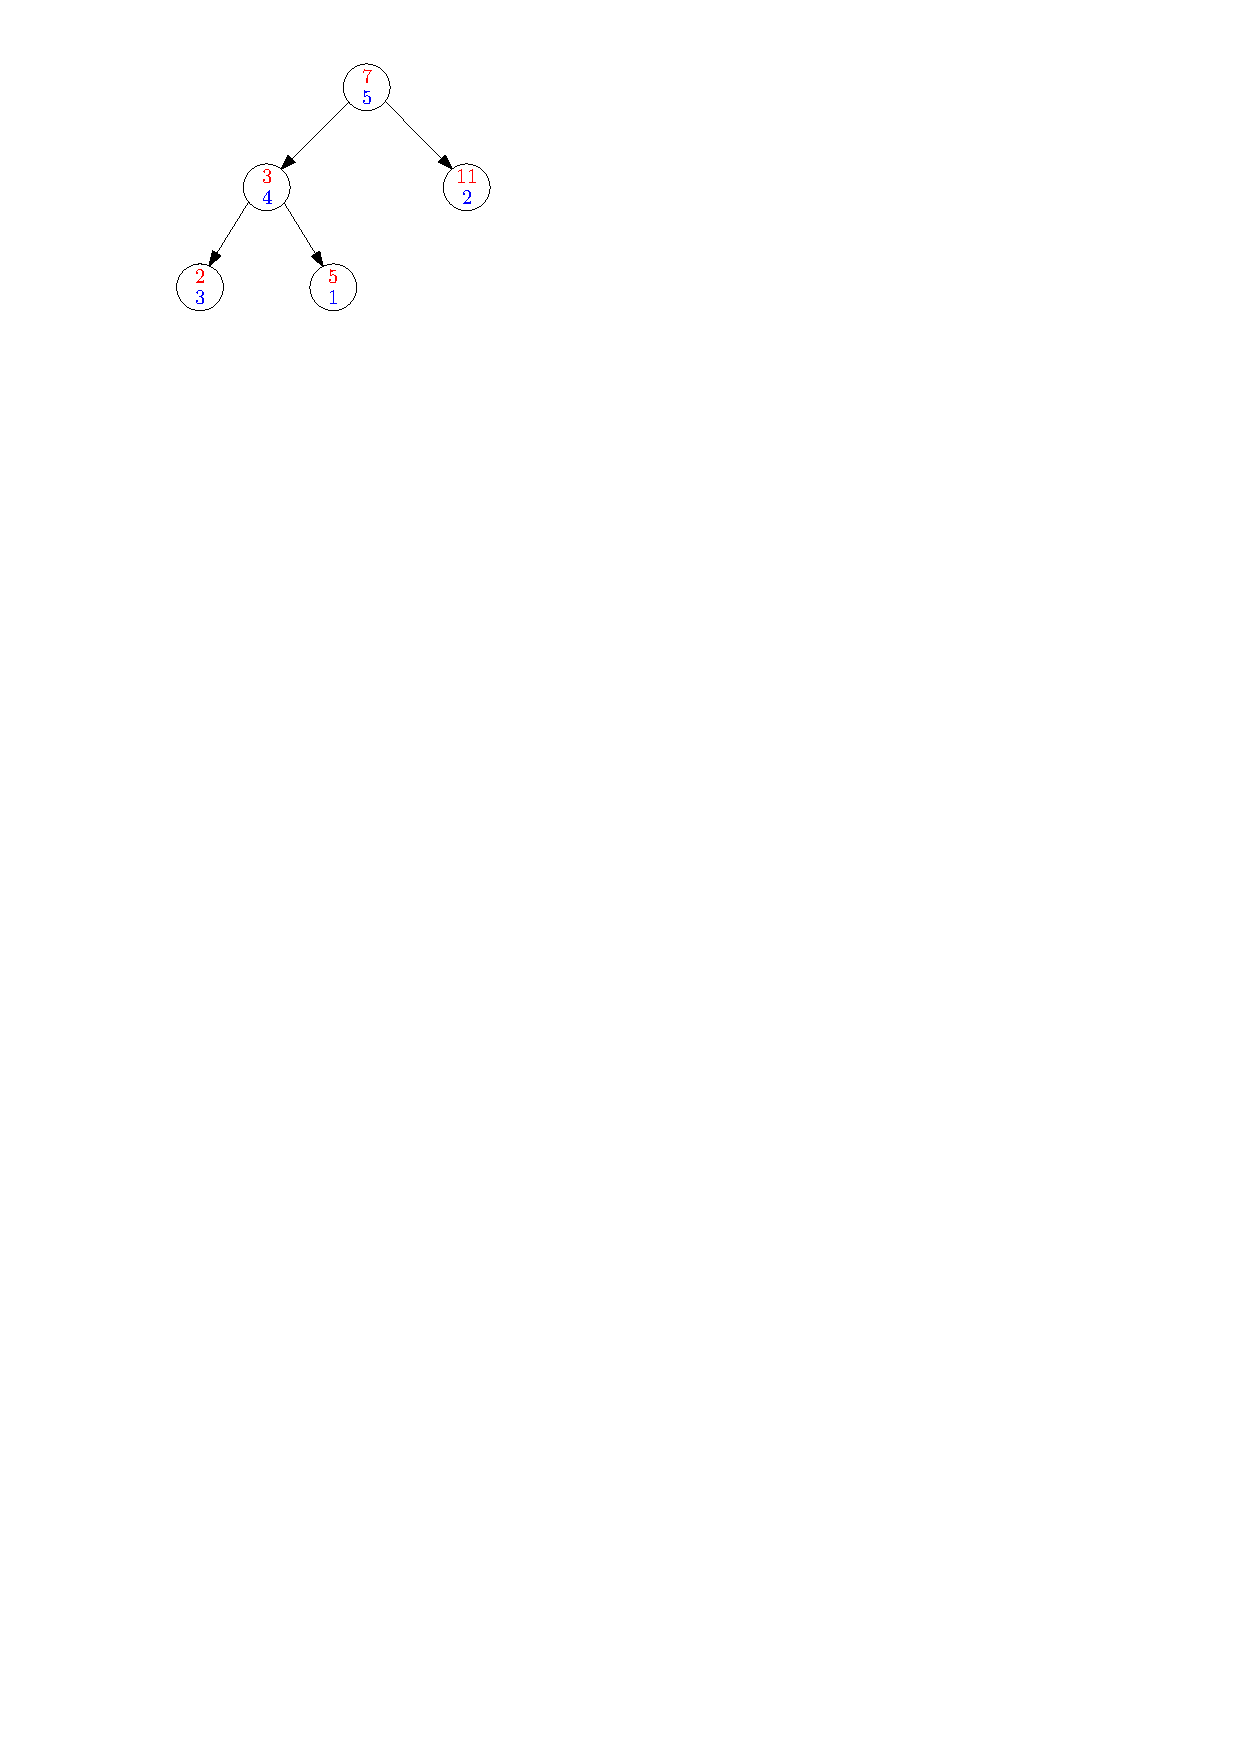
\includegraphics{img/Beispiel_Treap.pdf}
\caption{Beispiel eines Treaps - Schlüssel in rot, Priorität in blau}
\label{fig:exampletreap}
\end{figure}


\section{Existenz eindeutiger Treaps}
\label{sec:uniquetreaps}

\begin{satz}
Für jede Menge $S = \{(k_1,p_1), \dots, (k_n, p_n)\}$ von Schlüssel-Priorität-Paaren mit paarweise unterschiedlichen Schlüsseln und Prioritäten existiert genau ein gültiger Treap.
\end{satz}
\begin{beweis}[Beweis per Induktion über $n = |S|$]
\noindent\textbf{IA:} ($n = 0$) trivial

\noindent\textbf{IS:} ($n \to n+1$)
Sei $t = (k_j, p_j)$ das Paar mit der höchsten Priorität.
Dieses Element muss dann an der Wurzel des Treaps stehen.
Alle Elemente aus $M_< := \{(k_i, p_i) \in S \mid k_i < k_j\}$, die also einen kleineren Schlüssel als die Wurzel besitzen, müssen im linken Teilbaum liegen, analog gilt dies für die Elemente mit größerem Schlüssel als $t$.
Beide Teilbäume sind ebenfalls Treaps und sind nach der Induktionsvorraussetzung eindeutig bestimmt.
\end{beweis} %TODO: Bild

Dieser Satz zeigt, dass die Reihenfolge, in der die Knoten eingefügt werden, beliebig sein kann -- am Ende kommt immer der gleiche Treap heraus.
Wenn wir den Baum optimal für eine gegebene Menge an Schlüsseln balancieren wollen, ist es wichtig, die Prioritäten richtig zu wählen.
Hier kommt die Randomisierung ins Spiel:
Dadurch, dass zufällig gewählte Prioritäten dem Treap eine zufällige -- und damit wahrscheinlich balancierte -- Form geben, sind sie ideal für Treaps.
Man kann die Prioritäten effizient beim Einfügen eines Knotens durch einen Zufallsgenerator oder implizit durch eine Hashfunktion generiert werden.

\section{Implementierung}
\label{sec:implementing}
\subsection{Rotation}
\label{sec:rotation}
Bei den Update-Operationen werden Baumrotationen benutzt, um Knoten im Treap zu verschieben.
Dabei wird die Suchbaumeigenschaft beibehalten, während die relative Position zweier Knoten bezüglich der Prioritäten vertauscht wird.
Dazu muss darauf geachtet werden, dass man immer nur in Richtung des nach Priorität kleineren Kindknotens rotiert wird, sonst wird ein ganzer Teilbaum falsch positioniert.
In den folgenden Algorithmen wird verwendet, dass Knoten nach oben oder unten rotiert werden.
Dies bedeuted, dass der Baum so rotiert wird, dass sich der entsprechende Knoten nachher über seinem Elternknoten bzw. unter einem seiner Kindknoten befindet.
Beispielsweise wird der rote Knoten in Abbildung~\ref{fig:rotation} durch eine Rechtsrotation um sich nach unten rotiert und durch eine Linksrotation um den blauen Knoten nach oben rotiert.
\begin{figure}
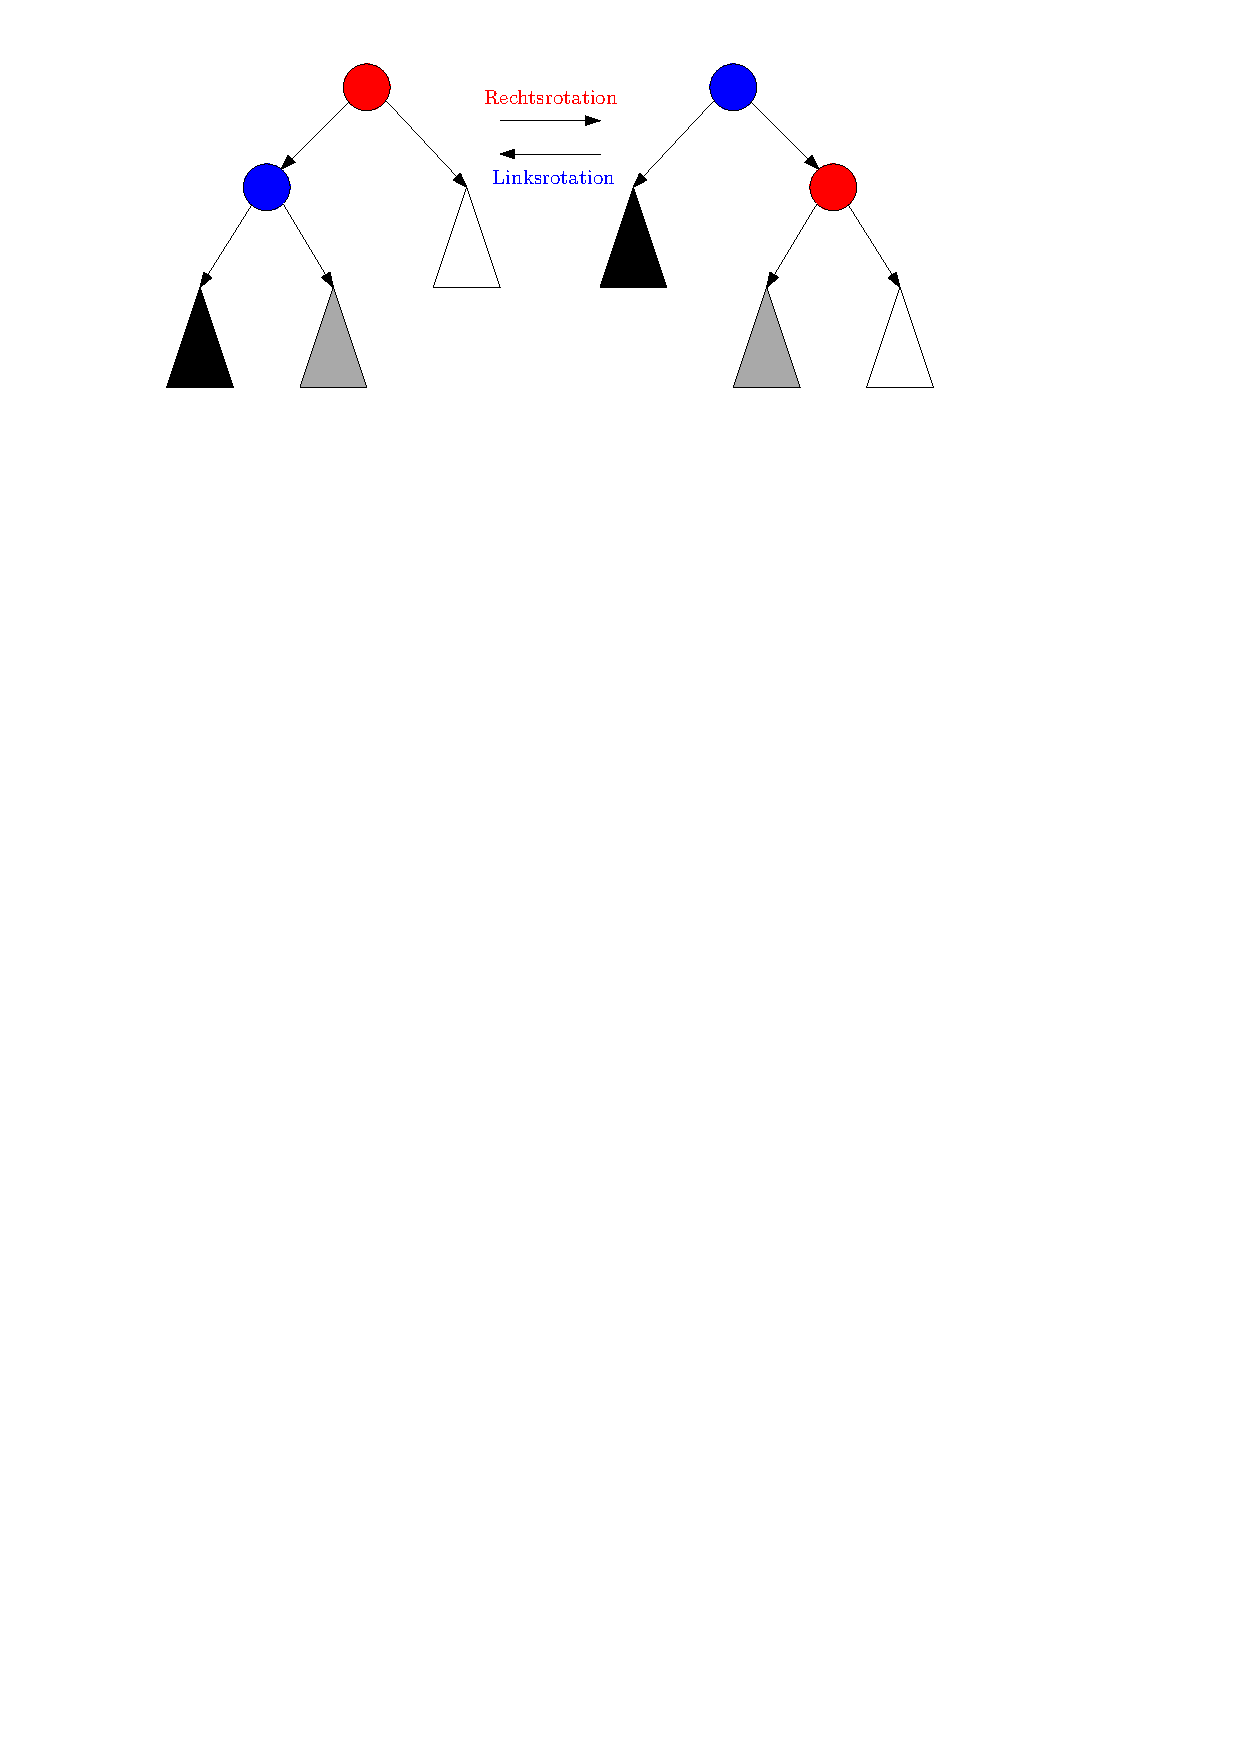
\includegraphics{img/Tree_Rotation_color.pdf}
\caption[Rotation eines Baums]{Rotation eines Baums}
\label{fig:rotation}
\end{figure}

\subsection{Find}
\label{sec:find}

Find wird genau wie bei binären Suchbäumen durchgeführt.

\subsection{Insert}
\label{sec:insert}

\begin{algorithm}[H]
	\Ein{Knoten $i$, Treap $S$}
		Füge $i$ als Blatt in $S$ ein \;
		\While{$i$.parent.prio $<$ $i$.prio}{
			Rotiere $i$ nach oben \;
		}
	\caption{Insert($i$, $S$)}
\end{algorithm}

\subsection{Delete}
\label{sec:delete}

\begin{algorithm}[H]
	\Ein{Schlüssel $k$, Treap $S$}
		\SetKw{Not}{not}
		\While{\Not istBlatt($i$)}{
			Rotiere $i$ nach unten \;
		}
		Lösche Blatt $i$ aus $S$ \;
	\caption{Delete($k$, $S$)}
\end{algorithm}

\subsection{Join}
\label{sec:join}

\begin{algorithm}[H]
	\Ein{Treaps $S_1, S_2$, Knoten $i$}
	\Aus{Treap $S$}
		\SetKw{Or}{or}
		$i$.left $\gets S_1$ \;
		$i$.right $\gets S_2$ \;
		\While{$i$.prio $<$ $i$.left.prio\\ \Or $i$.prio $<$ $i$.right.prio}{
			Rotiere $i$ nach unten \;
		}
		\Return $i$
	\caption{Join($S_1$, $i$, $S_2$)}
\end{algorithm}

\subsection{Merge}
\label{sec:merge}

\begin{algorithm}[H]
	\Ein{Treaps $S_1, S_2$}
	\Aus{Treap $S$}
		$i$ $\gets$ Find($\infty$, $S_1$) \tcp{Maximum}
		Delete($i$, $S_1$) \;
		\Return Join($S_1$, $i$, $S_2$) \;
	\caption{Merge($S_1$, $S_2$)}
\end{algorithm}

\subsection{Split}
\label{sec:split}

\begin{algorithm}[H]
	\Ein{Treap $S$, Schlüssel $k$}
	\Aus{Treaps $i$.left, $i$.right}
		Delete($k$, $S$) \tcp{falls existent}
		$i \gets (k, \infty)$ \;
		Insert($i$, $S$) \;
		\Return $i$.left, $i$.right;
	\caption{Split($k$, $S$)}
\end{algorithm}

\section{Laufzeitanalyse}
\label{sec:runtime}
Zur Laufzeitanalyse führen wir so genannte \emph{Mulmuley-Spiele} ein.
Diese werden wir analysieren und dadurch die Tiefe von Knoten in einem Treap und die Anzahl der benötigten Rotationen beim Löschen berechnen.
Das genügt, um die Laufzeit aller Operationen zu erhalten.

\subsection{Mulmuley-Spiele}
\label{sec:mulmuley}
Für ein Mulmuley-Spiel werden folgende disjunkte Mengen definiert:
\begin{itemize}
    \item Eine Menge $P = \{P_1, P_2, \dots, P_p\}$ von $p$ \emph{Spielern},
    \item eine Menge $S = \{S_1, S_2, \dots, S_s\}$ von $s$ \emph{Stoppern},
    \item eine Menge $T = \{T_1, T_2, \dots, T_t\}$ von $t$ \emph{Triggern},
    \item eine Menge $B = \{B_1, B_2, \dots, B_b\}$ von $b$ \emph{Zuschauern}.
\end{itemize}
Die Elemente aus $P \cup S$ seien aus einem total geordnetem Universum, und dabei sollen die Spieler kleiner sein als die Stopper.
Die Mengen $T$ und $B$ können beliebig sein.
Bilde eine Menge $X$, indem man mehrere dieser vier Mengen vereinigt und ziehe aus dieser zufällig Elemente ohne Zurücklegen.
Man zählt dabei die Anzahl der Spieler, die größer sind als alle bisher gezogenen Spieler, wobei Stopper ebenfalls als Spieler gezählt werden.
Der Wert eines Spieles entspricht dem erwarteten Wert für diese Anzahl und ist damit abhängig von der Kardinalität der einzelnen Mengen.
In dieser Arbeit werden 3 Varianten der Mulmuley-Spiele vorgestellt:
In Spiel A besteht die Menge $X$ aus den Spielern $P$ und den Zuschauern $B$.
Gezogen wird solange die Menge $X$ nicht leer ist.
In Spiel C besteht die Menge $X$ aus den Spielern $P$, den Stoppern $S$ und den Zuschauern $B$,
Gezogen wird solange bis der erste Stopper gezogen wurde.
In Spiel D besteht die Menge $X$ aus den Spielern $P$, den Triggern $T$ und den Zuschauern $B$.
Gezogen wird solange die Menge $X$ nicht leer ist, allerdings fängt man erst mit dem Zählen an, wenn der erste Trigger gezogen wurde.

Der Wert $A^p$ von Spiel A mit $p$ Spielern beträgt $H_p$.
Dabei ist $H_p := \sum_{i=1}^p 1/p$ die p-te harmonische Zahl und es gilt $H_p \in \Theta(\log p)$.
Der Wert $C_s^p$ von Spiel B mit $p$ Spielern und $s$ Stoppern beträgt $1 + H_{s+p} - H_s$.
Der  Wert $D_t^p$ von Spiel C mit $p$ Spielern und $t$ Triggern beträgt $H_p + H_t - H_{t+p}$.~\cite{RandAlg}

\subsection{Laufzeit von Delete}
\label{sec:delruntime}
In diesem Unterabschnitt wird die Laufzeit einer Delete-Operation analysiert.
Dies ist ausreichend, da Insert genau den umgekehrten Ablauf hat wie Delete (\glqq Delete rückwärts\grqq), deshalb die gleiche Laufzeit hat, und die restlichen Operationen mit Hilfe einer konstanten Anzahl von Insert und Delete implementiert werden können.

Die Ausführung von Delete besteht aus 2 Phasen:
Zuerst wird der zu löschende Knoten im Treap gesucht, um dann in der zweiten Phase bis nach unten rotiert zu werden.
Die Laufzeit der ersten Phase hängt linear von der Tiefe des gesuchten Knotens im Baum ab.
Der Knoten wird in der zweiten Phase entlang des linken \emph{Grats} des rechten Teilbaums und des rechten Grats des linken Teilbaums nach unten rotiert.
Der linke/rechte Grat eines Baums ist definiert als der Weg, den man erhält, wenn man von der Wurzel aus immer zum linken/rechten Kindknoten absteigt.
Also ist die Laufzeit der zweiten Phase proportional zur Summe dieser beiden Grate.

Sei $X$ mit $\left|X\right| = n$ die Menge aller Knoten in einem Treap.
Sei $x$ ein Knoten mit Rang $r$, d.h. es gibt $r$ Knoten, deren Schlüssel nicht größer sind, als der von $x$.
Sei $X_\leq$ die Menge aller $r$ Knoten mit Schlüssel kleiner oder gleich $k(x)$.
Analog definiere $X_\geq$.
Zur Analyse beginnen wir mit einem leeren Treap und fügen seine Knoten nach absteigender Priorität ein.
Dies ergibt, wie oben gezeigt, genau den zu analysierenden Treap, wobei Knoten immer nur als Blatt eingefügt werden und keine Rotationen erforderlich sind.
Wie in Randomized Algorithms~\cite{RandAlg} gezeigt, sind die Knoten aus $X_\leq$, die sich entlang des Suchpfades von $x$ befinden, genau die Knoten, die zu dem Zeitpunkt, in dem sie eingefügt werden, die größten aus $X_\leq$ sind.
Möchte man die Anzahl dieser Knoten zählen, spielt man im Prinzip Spiel A mit $P = X_\leq$ und $B = X \setminus X_\leq$.
Damit ergibt sich ein erwartete Anzahl von $H_{\left|P\right|} = H_r$.
Betrachtet man auch die Knoten entlang des Suchpfades aus $X_\geq$, so ergibt sich aus Symmetriegründen eine erwartete Tiefe von $H_r + H_{n-r+1} - 1 \in O(\log n)$ für den Knoten $x$.
Eine Visualisierung der Korrespondenz von Treap und Spiel A findet man in Abbildung~\ref{fig:proofgamea}.
\begin{figure}
    \centering
    \includegraphics[page=10,width=\textwidth]{img/Laufzeit_Beweis.pdf}
    \caption[Beispiel: Treap mit Spiel A]{Beispiel für einen Treap und das zugehörige Spiel A.
    Dabei wird die Tiefe des Knoten mit dem Schlüsselwert $6$ analysiert.
    Die ausgegrauten Kästchen mit den Werten $7$, $8$ und $9$ stellen Zuschauer dar.}
    \label{fig:proofgamea}
\end{figure}
Ähnlich kann man auch für die Anzahl der Rotationen argumentieren.
Hierbei spielt man Spiel D mit $P = X_\leq \setminus \{x\}$, $T = \{x\}$ und $B = X \setminus X_\leq$, das den Erwartungswert $H_{r-1} + H_1 - H_r = 1 - 1/r$ hat.
Für die Gesamtzahl der Rotationen ergibt sich damit erwartet $2 - 1/r - 1/(n-r+1) < 2$.

\chapter{Fazit}
\label{sec:closing}
% Vorteil ggü naiver BT: Balancing -> Laufzeit, gerade, wenn Elemente in auf-/absteigender Reihenfolge eingefügt werden
% Vorteil ggü det. balancierter BT: einfache Implementierung, keine weiteren Informationen/Speicher nötig -> Hashfunktion
% Tabelle mit Laufzeitvergleich
Die in dieser Arbeit vorgestellten Treaps stellen eine gute Option zum Verwalten geordneter Mengen dar.
Gegenüber einfachen binären Suchbäumen haben Treaps den Vorteil, dass sie balanciert werden, was insbesondere dann eine Rolle spielt, wenn Elemente häufig in auf-/absteigender Folge eingefügt werden.
Gegenüber anderen (deterministischen) balancierten Suchbäumen haben Treaps den Vorteil, dass die Implementierung einfach ist.
Außerdem ist es möglich, keinen zusätzlichen Speicherplatz für Balancierungsinformationen zu verwenden, wenn man statt explizite Prioritäten anzugeben auf eine Hashfunktion setzt.
Allerdings ist die schnelle Laufzeit bei Treaps nicht garantiert, sondern nur sehr unwahrscheinlich, da es sich um einen Erwartungswert handelt.
Abschließend sei hier nochmal der direkte Vergleich der Laufzeiten dargestellt:

\vspace{1em}
% \begin{table}
% \centering
% \label{tab:treapvsbinarytree}
\begin{tabular}{l | c | c }
        Methode & Treap & Binärbaum\\
        \hline
        Insert$(i, S)$ & $O(\log n)$ & $O(h)$ \\
        Delete$(k, S)$ & $O(\log n)$ & $O(h)$ \\
        Find$(k, S)$ & $O(\log n)$ & $O(h)$ \\
        $S$ = Join($S_1, i, S_2$) & $O(\log n + \log m)$ & $O(1)$ \\
        $S$ = Merge($S_1, S_2$) & $O(\log n + \log m)$ & $O(h_1 + h_2)$ \\
        $S_1, S_2$ = Split$(k, S)$ & $O(\log n + \log m)$ & $O(h)$
        \end{tabular}
% \caption[Laufzeiten Treap vs. Binärbaum]{Laufzeitvergleich zwischen Treaps (Erwartungswert) und binären Suchbäumen (worst case).}
% \end{table}

Die Variablen $n$ bzw.\ $m$ stehen hierbei für die Anzahl der Elemente in den jeweiligen Treaps; die Variablen $h$, $h_1$ und $h_2$ geben die Höhe des Binärbaums an.





\bibliographystyle{mybabalpha-fl}
\bibliography{mybib}

\end{document}
